% #############################################################################
% This is Chapter 4
% !TEX root = ../main.tex
% #############################################################################
% Change the Name of the Chapter i the following line
\fancychapter{End-to-End children automatic speech recognition}
\label{chap:4}
\cleardoublepage
%\section{Introduction}
% End2End better and better
The efficacy demonstrated in incorporating \ac{DNN} within \ac{HMM-DNN} setups has motivated a widespread adoption of deep learning techniques in the \ac{ASR} field. Notably, this increased interest is underscored by the recent achievements obtained with end-to-end models, which have exhibited superior performance compared to traditional hybrid \ac{HMM-DNN} systems across a diverse array of speech recognition tasks \cite{zeyer2019comparison,zeineldeen2022Conformer}.
%The success observed in the application of deep learning within \ac{HMM-DNN} setups has motivated an increased utilisation of deep learning methods for \ac{ASR}. Notably, end-to-end models have recently demonstrated their capability to surpass hybrid \ac{HMM-DNN} systems across diverse speech recognition tasks \cite{zeyer2019comparison,zeineldeen2022Conformer}. 
The primary advantage of end-to-end speech recognition systems lies in the merging of the entire training pipeline within a single neural network, mitigating potential behavioural inconsistencies that may arise between the independent training of the different modules.
However, the application of the end-to-end paradigm in the realm of children's \ac{ASR} is a relatively recent development and has encountered limited exploration \cite{gelin2021endtoend,sri_end2end,chen2020data,ng2020cuhk}. Indeed, end-to-end models require a larger amount of data to achieve the desired robustness and flexibility, a condition that is often not met in the case of children's speech. Additionally, the merging of different components within end-to-end models contributes to an increased demand for trainable parameters. Consequently, training end-to-end models on small datasets becomes more challenging \cite{luscher2019rwth}. Despite these challenges, the exploration of end-to-end models holds promise for pushing the boundaries of the state-of-the-art in children's \ac{ASR}.



As discussed in Section \ref{section:SOTAE2E}, the increased interest in end-to-end speech recognition has led to the development of several architectures, including recurrent neural networks \cite{soltau2016neural}, neural transducers \cite{battenberg2017exploring}, and the Transformer architecture \cite{vaswani2017attention}. Notably, among these architectures, the Transformer stands out for its ability to consistently yield state-of-the-art results in large-vocabulary speech recognition. This effectiveness is not limited to adult speech but also extends to the domain of children's speech \cite{gelin2021endtoend,sri_end2end}. %The Transformer's adaptability and robustness make it a noteworthy candidate for advancing the field of end-to-end speech recognition, particularly in the context of children's \ac{ASR}.



Within this chapter, we will present the Transformer design, alongside the Conformer—an improved iteration of the Transformer architecture specifically created for speech-related tasks. Building on prior research that demonstrated the efficacy of Transformer-based models in children's \ac{ASR} \cite{gelin2021endtoend,sri_end2end}, particularly when fine-tuned from pre-trained adult models, our goal is to provide a comprehensive understanding of the various components within these architectures and their roles in achieving optimal \ac{TL} performances. To this end, we introduce the concept of \textit{partial fine-tuning}, a method where only specific components of the architecture are adapted during \ac{TL}. The aim of this work is to identify the essential elements underlying the success of transformer-based models during fine-tuning. This knowledge is essential for the further refinement and improvement of methods specifically designed for children's \ac{ASR}. The objective of this chapter is to address the following research questions: \textit{Can we furhter improve full end-to-end model fine-tuning of children \ac{ASR} by adapting part of the model? Particularly, what are the most important components to fine-tune?}
\section{Transformer model}
\label{sec:trans_archi}

\begin{figure}[ht]
    \centering
    \includegraphics[width=1\textwidth]{imgs/Transformer_archi.png}
    \caption{Architecture of the standard Transformer \cite{vaswani2017attention}. a) scaled dot-product attention, b) multi-head self-attention, c) Transformer-Encoder, d) Transformer-Decoder.}
    \label{fig:Transformer_archi}
\end{figure}
% Explain Transformer
Introduced in 2017 by Vaswani \textit{et al.} \cite{vaswani2017attention}, the Transformer architecture is a sequence-to-sequence Encoder-Decoder model that relies solely on attention mechanisms, completely discarding the use of recurrence and convolutions. This design choice addresses challenges such as vanishing gradient issues commonly associated with recurrent neural networks. Another notable difference with recurrent neural networks is that the Transformer computes the dependencies between each pair of positions simultaneously, rather than one by one, by directly encoding the position in the sequence. This enables more parallelisation and therefore a faster training process.

Since its introduction, the Transformer architecture had a tremendous impact across various domains, including \ac{NLP} \cite{Bert,brown2020language}, computer vision \cite{dosovitskiy2020image}, and speech processing \cite{dong2018speech}. The Transformer's capacity to capture intricate dependencies and patterns in sequences has established it as a popular architecture in the deep learning field, contributing to advancements and breakthroughs across various applications, such as ChatGPT \cite{bahrini2023chatgpt} or Dall-E \cite{ramesh2021zero}.

The Transformer Encoder-Decoder architecture, as depicted in Figure \ref{fig:Transformer_archi}, consists of an Encoder (c) and a Decoder (d). Prior to entering the Encoder or Decoder, both inputs and targets undergo processing through an embedding layer. This involves the use of learned embeddings to convert input tokens and output tokens into vectors of dimension $d_{\text{model}}$. 
% Positional embedding
Since the Transformer model contains no recurrence and no convolution mechanisms, information about the relative or absolute position of the tokens must be injected into the sequence to allow the model to make use of the order of the sequence. To achieve this, information about the relative or absolute position of the tokens is obtained through the summation of the input/output embedding and the positional embedding. While various alternatives for positional encodings were used, Vaswani \textit{et al.} \cite{vaswani2017attention} proposed the use of sinusoidal and cosine functions with different frequencies, as follows:

\begin{align}
    PosEnc_{(pos,2i)} = \sin(pos/10000^{2i/d_{\text{model}}})\\
    PosEnc_{(pos,2i+1)} = \cos(pos/10000^{2i/d_{\text{model}}})
\end{align}
Where $pos$ is the current token or label position and $i$ is the dimension.
 

%Encoder
The Encoder's primary objective is to transform the input sequence $X = x_1, \dots, x_T$ into a series of continuous ``hidden" representations $Z = z_1, \dots, z_T$. The Encoder is structured as a stack of $L$ identical layers, each comprising two sub-modules: the \ac{MHSA} and the position-wise fully connected \ac{FFN}. Each of these modules is followed by a normalisation with a residual connection.

%Decoder
Subsequently, the continuous ``hidden" representations $Z$ are fed into the Decoder. The Decoder is responsible for constructing an output sequence $Y = y_1, \dots, y_N$ one element at a time. At each time step, the Decoder receives both the Encoder outputs and the last Decoder output in an auto-regressive manner. Similarly to the Encoder, the Decoder is composed of a stack of $J$ identical layers. Nevertheless, in comparison to the Encoder, the Decoder encompasses a third sub-module, which performs \ac{MHA} over the output of the Encoder stack. The self-attention sub-module in the Decoder stack is modified to prevent positions from attending to subsequent positions. This masking combined with a modified \ac{MHA} prevents the attention from using subsequent positions, ensuring that the prediction at time-step $i$ solely depends on the previous $< i$ time-steps.

%MHSA 
The \ac{MHA} module relies on scaled dot-product attention \cite{vaswani2017attention}, as illustrated in Figure \ref{fig:Transformer_archi}(a). Scaled dot-product attention focuses on determining how relevant a particular token is with respect to other tokens in the sequence and is defined as follows:

\begin{align}
\text{Attention}(Q, K, V) = \text{softmax}\left(\frac{QK^T}{\sqrt{d_k}}\right)V
\label{equation:attention}
\end{align}


Here, the input consists of queries $Q$, keys $K$ of dimension $d_k$, and values $V$ of dimension $d_v$. The dot product of the query with all keys is divided by $\sqrt{d_k}$, and the result passes through a softmax function to obtain attention weights. The attention weights are then multiplied with the values $V$. When $d_k$ is large, the scaling  $\frac{1}{\sqrt{d_k}}$ restrains the dot product from growing large in magnitude. Note that the \ac{MHSA} is a specific case of \ac{MHA} where $K$, $V$, and $Q$ are all the same input of the module. 

Instead of performing a single scaled dot-product attention, \ac{MHA} modules linearly project $h$ times $K$, $V$, and $Q$ with different, learned, linear projections to dimensions $d_k$, $d_k$, and $d_v$ respectively. The attention function \ref{equation:attention} is then applied in parallel to each of the $h$ projected versions. The output of each of the $h$ attention functions, of dimension $d_v$, is concatenated and projected one final time, as depicted in Figure \ref{fig:Transformer_archi}(b). Each of the $h$ attention functions is called a head, while the overall is called \ac{MHA} or \ac{MHSA} if $K$, $V$ and $Q$ are the same. More formally:

\begin{align}
\text{MultiHead}(Q, K, V) = \text{Concat}(\text{head}_1, \dots, \text{head}_h)W^O
\end{align}
where
\begin{align}
\text{head}_i = \text{Attention}(QW_i^Q, KW_i^K, VW_i^V)
\end{align}
and the different projection matrices are $W_i^Q \in \mathbb{R}^{d_{\text{model}} \times d_k}$, $W_i^K \in \mathbb{R}^{d_{\text{model}} \times d_k}$, $W_i^V \in \mathbb{R}^{d_{\text{model}} \times d_v}$, and $W^O \in \mathbb{R}^{hd_{v} \times d_{\text{model}}}$.


% \ac{FFN}
Furthermore, in addition to the attention modules, each Transformer layer within the Encoder and Decoder encompasses a \ac{FFN} module. This network is applied to each position separately and identically, and it consists of two linear transformations with a \ac{ReLU} activation in between. While attention captures interdependencies between the elements of the sequence regardless of their position, the \ac{FFN} non-linearly transforms each input token independently:

\begin{align}
    FFN(x) = max(0,xW_1 + b_1)W_2 + b_2
    \label{equation:FFN}
\end{align}
With $W_1 \in \mathbb{R}^{d_{model} \times d_{FFN}}$, $b_1 \in \mathbb{R}^{d_{FFN}}$, $W_2 \in \mathbb{R}^{d_{FFN} \times d_{model}}$ and $b_2 \in \mathbb{R}^{d_{model}}$. Typically $d_{FFN}$ is usually set to $4 \times d_{model}$.

\section{Conformer model}
\label{sec:Conformer}
\begin{figure}[h]
    \centering
    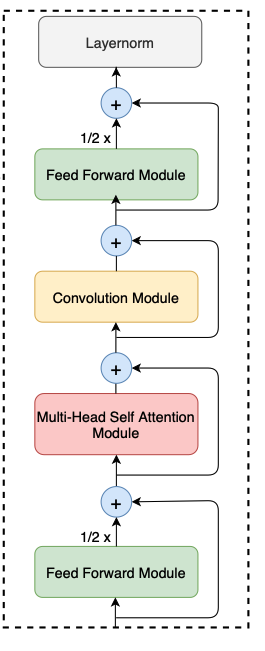
\includegraphics[scale=0.4]{imgs/ConformerLayer.png}
    \caption{Architecture of a Conformer layer}
    \label{fig:Conformer_archi}
\end{figure}

\begin{figure}[h]
    \centering
    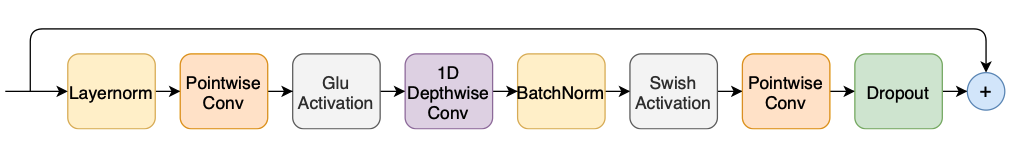
\includegraphics[width=1\textwidth]{imgs/ConvolutionModule.png}
    \caption{Convolution module in the context of a Conformer layer}
    \label{fig:convModule}
\end{figure}
Transformers are recognised for their effectiveness in capturing global information within sequential tasks, a capability attributed to the attention mechanism. Conversely, \acp{CNN} networks excel in capturing local features within data. To leverage the complementary strengths of both architectures, various approaches have been explored \cite{bello2019attention,yang2019convolutional}, and the Conformer architecture \cite{gulati2020conformer} stands out as a notable combination of Transformers and \acp{CNN}.

This combination involves incorporating \acp{CNN} into the conventional Transformer architecture, as depicted in Figure \ref{fig:Conformer_archi}. Specifically, a Conformer block comprises four modules arranged sequentially: a \ac{FFN} module, a \ac{MHSA} module, a convolution module, and a second \ac{FFN} module. Notably, the Conformer block features two \ac{FFN} modules sandwiching the \ac{MHSA} module and the Convolution module. This design is inspired by the Macaron-Net \cite{lu2019understanding}, which advocates replacing the original \ac{FFN} in the Transformer block with two half-step \ac{FFN} modules—one before the attention layer and one after. Similar to Macaron-Net, half-step residual weights are employed for the \ac{FFN} modules. More formally, for an input $x_i$ to a Conformer block $i$, the output $y_i$ of the block is defined as follows:


\begin{align}
    \begin{split}
    \tilde{x_i} = x_i + \frac{1}{2}FFN(x) \\
    x_i^{\prime} =\tilde{x_i} + MHSA(\tilde{x_i}) \\
    x_i^{\prime\prime} = x_i^{\prime} + Conv(x_i^{\prime}) \\
    y_i = LayerNorm(x_i^{\prime\prime} + \frac{1}{2}FFN(x_i^{\prime\prime}))
    \end{split}
\end{align}

More specifically, the convolution module used in a Conformer layer is inspired by the work of Wu \textit{et al.} \cite{wu2020lite} and illustrated in Figure \ref{fig:convModule}. It starts with a gating mechanism \cite{dauphin2017language} involving a pointwise convolution and a \ac{GLU} activation function. Subsequently, a single 1-D depthwise convolution layer is employed. Finally, this 1-D depthwise convolution is followed by a Batch-normalisation and then a Swish activation layer \cite{Prajit2017Searching}.

In summary, Conformers differentiate themselves from Transformers by incorporating convolutional layers to capture local dependencies in addition to the self-attention mechanisms. This design makes Conformers especially suitable for tasks dealing with sequential data, such as speech processing, where the temporal aspect of information is crucial. Notably, this architecture demonstrates improved accuracy compared to previous approaches on datasets like LibriSpeech \cite{gulati2020conformer}.


\section{Exploring transfer learning efficacy for Transformer-based models}
% Explain motivation 
The end-to-end paradigm has emerged as the state-of-the-art approach for many adult speech datasets, by integrating all components of the traditional \ac{HMM}-based \ac{ASR} pipeline, such as acoustic, pronunciation, and language models, into a single neural network. However, this unified neural network design results in a substantial increase in the number of parameters. While handling a large number of parameters is feasible when training on extensive adult data, it poses challenges for smaller children's speech datasets. This limitation has been underscored in previous works \cite{sri_end2end,gelin2021endtoend}, where end-to-end models trained on children's speech from scratch were found to be less accurate than traditional hybrid \ac{HMM-DNN} systems.

%TL
In light of this challenge, \ac{TL} emerges as a promising strategy to address the problem of training large amounts of parameters for a limited-size children's dataset. The key idea is to leverage pre-trained adult models, which are trained on extensive datasets of adult speech. These pre-trained models are adapted to the specific characteristics of children's speech through a re-training phase using the children's dataset. Notably, this adaptation process relies on the use of the knowledge gained during the pre-training phase, eliminating the need to train models from scratch and making the process more manageable for smaller target datasets. The efficacy of the \ac{TL} approach for children \ac{ASR} has been demonstrated not only in traditional \ac{HMM-DNN} approaches, as discussed in the previous Chapter \ref{chap:Chapter3} and supported by existing literature \cite{shivakumar2020transfer}, but also in modern end-to-end paradigms \cite{sri_end2end,gelin2021endtoend}.

% Transfer learning on the entire model might not be effective
With the recent trend of increasing model complexity and parameter count, it becomes crucial to comprehend how these models perform when fine-tuned with limited downstream data. Training models with an expanding number of parameters on a relatively small dataset may potentially result in decreased performance. Consequently, a more detailed exploration of \ac{TL} for children's speech is needed to identify which parts of the network are more important in the fine-tuning process.

Moreover, the well-recognised issue of overparameterisation in large Transformer-based models, initially discovered in the \ac{NLP} field, adds an additional layer of complexity. Indeed, models like BERT \cite{Bert} have been acknowledged to be overparameterised in various studies \cite{kovaleva-etal-2019-revealing,michel2019sixteen}. Overparameterisation occurs when models have more parameters than necessary for a given task. Empirical observations suggest that certain components or layers of the architecture can be removed without compromising performance, and in some cases, may even lead to slight performance gains \cite{kovaleva-etal-2019-revealing,michel2019sixteen,ye2023partial}. In addition, the recognition of overparameterisation has paved the way for successful compression studies, including pruning and distillation techniques \cite{mccarley2019structured,sanh2019distilbert}. These approaches aim to address the challenges posed by an excessive number of parameters by reducing the model sizes without compromising performances. 

In view of the overparameterisation problem, there is a growing need for ablation studies, involving the systematic removal of components of the model, to understand which parts significantly contribute to performance \cite{shen2021partial,wang2021fine}. These studies, predominantly explored in the field of computer vision \cite{ye2023partial}, align with the Lottery Ticket hypothesis formulated by Frankle and Carbin \cite{frankle2018lottery}:

\begin{quote}
    \textit{``A randomly-initialised, dense neural network contains a subnetwork that is initialized such that—when trained in isolation—it can match the test accuracy of the original network after training for at most the same number of iterations''}.
\end{quote}

While ablation works have been studied in other fields, they remain under-explored for speech tasks. As a matter of fact, the recent successes of distillation and pruning techniques for speech models \cite{gandhi2023distilwhisper,chang2022distilhubert,peng23c_interspeech} suggest that overparameterisation is also present in \ac{ASR} models. Consequently, understanding the contribution of the different components of large-size models would not only help optimise model architectures for specific tasks but also reduce the computational demands of training and inference. This is particularly relevant in scenarios with resource constraints, such as limited computational power, memory, and training data. For example, in the context of children's \ac{ASR}, where data scarcity is a significant challenge, understanding how overparameterisation affects the model could pave the way for the development of more tailored and efficient models. %To this end, identifying which components of the network are the most crucial during fine-tuning could help reduce the number of trainable parameters. 
%Notably, the Transformer and Conformer architectures have exhibited promising results in \ac{ASR} applications, making them particularly compelling subjects for further investigation.


\subsection{Partial Transfer learning}
% Explain experiments
In this Chapter, our objective is to conduct a comprehensive exploration of \ac{TL}, specifically on end-to-end children's \ac {ASR}. Notably, previous research in this field has solely been focused on \ac{HMM-DNN} models, as illustrated by the work of Shivakumar \textit{et al.} \cite{shivakumar2020transfer}. This previous work provided recommendations for the development of better children's \ac{ASR} systems, but such a study is currently missing for the end-to-end paradigm, which further motivated our investigation. It is noteworthy that existing works on \ac{TL} on the end-to-end paradigm have solely focused on the entire model fine-tuning, leaving a notable gap in the understanding of the impact of fine-tuning individual components. 

Firstly, we perform a meticulous examination of the \ac{TL} process, specifically isolating the effects on individual components of the Encoder and Decoder, in comparison to the fine-tuning of the entire model in Transformer-based models. The prevailing hypothesis asserts that the Encoder is capturing acoustic information, while the Decoder encodes more linguistic information. Considering the important presence of acoustic variability in children's speech, our investigation extended to discern which layers of the Encoder are more relevant for achieving effective \ac{TL} and how many of them need to be fine-tuned.


Subsequently, our focus shifts to delineating the distinctive contributions of modules within both the Transformer and Conformer architectures during the fine-tuning process of adapting a pre-trained adult model to children's speech. Our approach called \textit{Partial Fine-Tuning}, aims to investigate the existence of a ``Lottery winning ticket" module specifically within the fine-tuning of a Transformer-based model.
In contrast to previous work, where the entire model or entire layers are fine-tuned, our granular analysis takes a unique approach by assessing the individual roles of key components, independently of the layers they are in. Namely \ac{MHSA}, \ac{FFN}, and normalisation layers for the Transformer and Conformer model in addition to the convolution modules for the Conformer. The objective is to gain insights into the necessity and impact of each module, allowing us to selectively and partially fine-tune the model using a small children's dataset. Therefore, we aim with this approach to require fewer trainable parameters while maintaining the model's effectiveness. Indeed, by departing from the conventional whole-model or whole-layer fine-tuning, our approach aims to optimise the utilisation of limited data resources, contributing to the development of more efficient and tailored models for children's \ac{ASR}.


\subsection{Experimental setup}
\label{section:methods_chapter4}

\subsection{Corpus}
\begin{table}[ht]
\centering
\begin{tabular}{c|c|c}
\hline
 Training & Validation     & Test   \\ \hline
60897 utterances  & 10044 utterances   & 4079 utterances \\ 
 566 speakers  & 79 speakers   & 91 speakers \\ 
 113 hours  & 18 hours   & 13 hours \\ \hline

\end{tabular}
\caption{My Science Tutor Children Speech Corpus statistics}
\label{tab:statistics_myst}
\end{table}
Given that the end-to-end paradigm involves encapsulating both the acoustic model and language model within the same network, careful consideration is essential when selecting the dataset for experimentation. Specifically, if the model is trained on a restricted set of repeated prompts, such as a dataset focused on reading tasks, it may learn and overfit to those specific prompts, potentially compromising its ability to recognise spontaneous speech and yielding unreliable results. In response to this concern, we decided to use the Boulder Learning My Science Tutor (MyST) corpus, a spontaneous children's speech dataset, as described in section \ref{section:children_corpora}. 

We want to emphasise that we employed the same data filtering and splits as the experiment previously reported using \ac{HMM-DNN} settings, as detailed in Section \ref{section:HMMDNNADULT2CHILD}. A summary of the corpus details is recapitulated in Table \ref{tab:statistics_myst}.

\subsection{Implementation details}
\label{section:TransformerConformerDetails}
% Transformer  and Conformer model description
All experiments were conducted using the SpeechBrain toolkit \cite{speechbrain}. The Transformer model encompasses 12 Transformer layers in the Encoder and 6 Transformer layers in the Decoder, all with a hidden dimension of 512. Similarly, the Conformer architecture featured 12 Conformer layers in the Encoder and 6 Transformer layers in the Decoder, with a hidden dimension of 512. Both configurations used 8 heads for all \ac{MHSA}, a \ac{FFN} hidden dimension of 2048, and a dropout rate of 0.1. These models were pre-trained on a large English adult speech corpus, specifically the entire LibriSpeech dataset \cite{librispeech}, comprising 1,000 hours of data. For reproducibility, these pre-trained models are publicly available\footnote{https://huggingface.co/speechbrain/ASR-Transformer-Transformerlm-librispeech\\ https://huggingface.co/speechbrain/ASR-Conformer-Transformerlm-librispeech}. Furthermore, for all experiments, the same Transformer language model was employed, trained on 10 million words from LibriSpeech transcriptions. Our training involved 30 epochs with a learning rate of $8 \times 10^{-5}$. Furthermore, in line with findings of previous work \cite{gelin2021endtoend}, a combination of \ac{CTC} and \ac{Seq2Seq} losses was used, with respective weights of 0.3 and 0.7.

\subsection{Encoder-Decoder Transfer learning}
\label{sec:ED_partial}
% Encoder - Decoder
\begin{table}
    \begin{center}
        \begin{tabular}{lcc}\hline
            Transformer    &   \ac{WER} $\downarrow$    & Trained parameters  \\ \hline
            Full model          & 12.99\% & 71.5M   \\
            Encoder only & \textbf{12.55\%} & 37.8M  \\
            Decoder only & 15.95\% & 25.2M  \\ \hline \hline
            Conformer    &    & \\ \hline
            Full model          & 12.28\% & 109M   \\
            Encoder only & \textbf{11.24\%} & 75.9M  \\
            Decoder only & 16.94\% & 25.2M  \\ \hline 

        \end{tabular}
    \end{center}
    \caption{Fine-tuning in isolation of the Encoder and Decoder for Transformer and Conformer architecture}
    \label{tab:EncoderDecoder}
\end{table}
Table \ref{tab:EncoderDecoder} summarises the results of the impact of isolating fine-tuning of the Encoder and Decoder components within Transformer and Conformer \ac{ASR} models. For the Transformer model, fine-tuning the entire model exhibits a \ac{WER} of 12.99\% using 71.5 million parameters. Isolating the Encoder component leads to an improved \ac{WER}, with 12.55\% \ac{WER} with a reduced parameter count of 37.8 million. In parallel, fine-tuning only the Decoder underperformed compared to the full model and Encoder only fine-tuning strategies by achieving a \ac{WER} score of 15.95\% with 25.2 million parameters.

Turning to the Conformer model, the full model achieves a \ac{WER} of 12.28\% with 109 million parameters updated. Isolating the \ac{TL} on the Encoder yields a remarkable improvement, resulting in a \ac{WER} of 11.24\% with a parameter count of 75.9 million. Conversely, when only the Decoder  is fine-tuned the performances degraded with a higher \ac{WER} of 16.94\% using 25.2 million parameters. Notably, the Conformer architecture consistently outperformed the Transformer across all configurations, emphasising its effectiveness for speech-related tasks. In addition, these results underscore the important role of the Encoder in both Transformer and Conformer \ac{ASR} models compared to the Decoder. Our results highlight the Encoder's role in capturing the inherent variabilities in children's acoustics. We hypothesise that the acoustics variabilities represent the most important source of variabilities as suggested by previous research \cite{TFchildren}.

% Layers wise
\begin{figure}
    \centering
    \subfigure[Results of the transfer learning layer-wise for the Transformer model]{\label{fig:transferTLTransformer}\includegraphics[width=\textwidth]{imgs/layerTL_Transformer.png}}
    \subfigure[Results of the transfer learning layer-wise for the Conformer model]{\label{fig:transferTLConformer}\includegraphics[width=\textwidth]{imgs/layerTL_Conformer.png}}
    \caption{Layers-wise up-way and down-way transfer learning experiment for Transformer and Conformer architecture}
    \label{fig:layerWISE}
\end{figure}

Recognising the pivotal role of the Encoder in the success of the fine-tuning process for children's \ac{ASR}, our investigation delves deeper to determine the specific layers that are the most important during this \ac{TL} process. To this end, we adopted a meticulous approach where we incrementally fine-tuned the Encoder by adding one layer at a time for each fine-tuning experiment. This layer-wise fine-tuning procedure is executed bidirectionally, encompassing both an up-ward trajectory, commencing from the input layer, and a down-ward trajectory, starting from the output layer of the Encoder. In other words, the up-ward trajectory involves progressively fine-tuning by adding one layer at a time for each experiment, starting from the input layer and systematically integrating subsequent layers towards the output layer of the Encoder. Conversely, the down-ward trajectory initiates fine-tuning from the output layer, systematically incorporating preceding layers towards the input layer at each experiment. The results of this layer-wise fine-tuning procedure for both the Transformer and Conformer architectures are presented in Figure \ref{fig:layerWISE}.

In both the Transformer and Conformer scenarios, a consistent pattern emerged. The addition of more layers was found to be consistently beneficial, with optimal performance stabilisation occurring when 10 layers out of the 12 are employed. We observed that it is more advantageous to use \ac{TL} from the top layers in the down-ward direction (i.e. those close to the output of the Encoder) compared to the bottom layers in the up-ward direction (i.e. those close to the input of the Encoder). The success of the up-ward trajectory, in contrast to the down-ward trajectory, indicates that the top layers of the Encoder are the most relevant to fine-tuning in the context of children's \ac{ASR}. This exploration of layer-wise fine-tuning sheds light on the dynamics of \ac{TL} within the Encoder, offering valuable insights into the targeted layers that significantly contribute to optimising the performance of children's \ac{ASR} models. 

\subsection{Modules Transfer learning}
% Block wise
\begin{table}
    \begin{center}
        \begin{tabular}{lcc}\hline
            \textbf{Transformer}    & WER  $\downarrow$   & Trained parameters \\ \hline
            Frozen pretrained & 25.04\% & -   \\
            Full model   & 12.99\% & 71.5M   \\ \hline
            Normalisation & 17.00\% & 57.9K  \\
            Attention & 12.19\% & 25.2M  \\
            FFN    & \textbf{11.84\%}     &  37.8M \\ \hline
            Normalisation$_{Encoder}$ & 17.75\% & 25.6K \\ 
            Attention$_{Encoder}$ & 12.83\% & 12.6M \\ 
            FFN$_{Encoder}$ & 12.20\% & 25.2M \\ \hline 
            Attention + FFN & 12.39\% & 63.0M \\
            Normalisation + FFN & 12.19\% & 37.9M \\
            Normalisation + Attention & 12.29\% & 25.3M\\ \hline \hline
            \textbf{Conformer}    &     & \\ \hline
            Frozen pretrained & 21.75\% & -   \\
            Full model   & 12.28\% & 109M   \\ \hline
            Normalisation & 15.61\% & 63.7K  \\
            Attention & 11.74\% & 28.4M  \\
            Convolution Module & 11.67\% & 9.7M \\
            FFN    & \textbf{11.10\%}     &  63M \\
            \quad $\hookrightarrow$ Module 1    & 11.44\%     &  25.2M \\
            \quad $\hookrightarrow$ Module 2    & 11.48\%     &  25.2M \\
            \quad $\hookrightarrow$ Up-linear ($W_1$)    & 11.47\%     &  31.5M \\
            \quad $\hookrightarrow$ Down-linear ($W_2$)    & 11.40\%     &  31.5M \\ \hline
            Normalisation$_{Encoder}$ & 15.88\% & 37.9K \\ 
            Attention$_{Encoder}$ & 11.91\% & 15.7M \\ 
            FFN$_{Encoder}$ & 11.17\% & 50.4M \\ \hline
            FFN + Attention & 11.20\% & 91.4M \\
            FFN + Convolution Module & 11.11\% & 72.7M \\
            FFN + Normalisation & 11.15\% & 63.1M \\
            Attention + Normalisation & 11.67\% & 28.4M \\
            Attention + Convolution Module & 11.44\% & 38.0M \\
            Convolution Module + Normalisation & 11.62\% & 9.7M\\ \hline
        \end{tabular}
    \end{center}
    \caption{Modules fine-tuning experiment}
    \label{table:ModulesTL}
\end{table}
The results of our \textit{partial transfer learning} experiments, focusing on fine-tuning specific components of Transformer and Conformer \ac{ASR} models for children's speech, are presented in Table \ref{table:ModulesTL}. We decomposed our experiments into three parts. Firstly, we fine-tuned components in both the Encoder and Decoder. Secondly, we partially fine-tuned only the components present in the Encoder, motivated by the results of the Encoder fine-tuning in Section \ref{sec:ED_partial}. Finally, we investigated different combinations of fine-tuning components in both the Encoder and Decoder. In addition to the \ac{WER} evaluation metric, we also display the number of trained parameters to evaluate the parameter cost of the different components. 

% Transformer
The baseline performance of the Transformer pre-trained model without any fine-tuning (corresponding to the \textit{Frozen-pretrained} line) yields a \ac{WER} of 25.04\%. In contrast, the fine-tuning of the entire Transformer model exhibits a noteworthy improvement, achieving a \ac{WER} of 12.99\% with 71.5 million parameters trained.

The fine-tuning of specific components reveals valuable observations. Applying \ac{TL} on the normalisation layers alone results in a modest improvement \ac{WER} of 17.00\% by using 57.9 thousand parameters. The fine-tuning of \ac{MHSA} modules outperforms normalisation and full fine-tuning, achieving a \ac{WER} of 12.19\% with a parameter count of 25.2 million. The most important improvement was observed with the \ac{FFN} modules, which attained a remarkable \ac{WER} of 11.84\% using 37.8 million parameters. Remarkably, both \ac{MHSA} and the \ac{FFN} modules, when fine-tuned individually, already outperform the full model performance. This implies that the decrease in the number of parameters, coupled with the significance of these modules, may play a substantial role in the enhanced performances of the fine-tuning process with a limited dataset.

%Conformer
Turning to the Conformer model, the baseline \ac{WER} without fine-tuning gives 21.75\%. In contrast, the full fine-tuning of the Conformer model yielded an improved \ac{WER} of 12.28\% with 109 million parameters.

Fine-tuning specific Conformer modules offers further granularity. First, the normalisation layers fine-tuning, in a similar way as observed in the Transformer configuration, yield a score of 15.61\% WER, with 63.7 thousand parameters. Then, \ac{MHSA} modules proved to be effective by already providing better results than the full full-tuning with a \ac{WER} of 11.74\%, by training 28.4 million parameters. The convolution modules outperformed the \ac{MHSA} with a \ac{WER} of 11.67\% with fewer parameters used, 9.7 million. However, as in the Transformer model, \ac{FFN} modules stand out significantly, demonstrating a \ac{WER} of 11.10\% with a parameter count of 63 million. Notably, all the \ac{MHSA}, convolution modules and \ac{FFN} modules, when fine-tuned in isolation, surpass the performance of the full Conformer model.

% \ac{FFN} wise

As the \ac{FFN} modules consistently proved to be the most relevant component to fine-tune for children's \ac{ASR}, irrespective of the configuration, we opted to delve deeper into the \ac{FFN} submodule. We identify two ways to subdivide the \ac{FFN} components of a Conformer model. The first split is along the macaron-style of a Conformer \ac{FFN} layer, which includes two modules—one before the \ac{MHSA} and one after the convolution module, referred to as Module 1 and Module 2, respectively. The second subdivision of a \ac{FFN} module involves focusing solely on the up-linear and down-linear components, denoted as $W_1$ and $W_2$ in Equation \ref{equation:FFN}. Using the first splitting, Module 1 and Module 2 achieve \acp{WER} of 11.44\% and 11.48\%, respectively, each by fine-tuning 25.2 million parameters. While the Up-linear and Down-linear submodules exhibit \acp{WER} of 11.47\% and 11.40\%, respectively, with parameter counts of 31.5 million. The subdivision of the \ac{FFN} modules did not result in better performance than their coupled usage. This underscores the significance of fine-tuning the full \ac{FFN} modules in Transformer-based end-to-end models.

% Encoder only
Based on the findings outlined of Section \ref{sec:ED_partial}, where the significance of fine-tuning the Encoder module for children's \ac{ASR} was highlighted, we investigated whether fine-tuning various components of Transformer and Conformer layers would yield better results when focused solely on the Encoder. It is important to note that for this experiment, we excluded the fine-tuning of Convolution modules, as they are already exclusively present in the Encoder within the Conformer architecture, in other words, $Convolution modules_{Encoder} = Convolution modules$. Our findings revealed that isolating the fine-tuning of Normalisation$_{Encoder}$, Attention$_{Encoder}$, and FFN$_{Encoder}$ modules solely within the Encoder resulted in minimal performance degradation compared to fine-tuning these modules in both the Encoder and Decoder. This slight discrepancy can be attributed to the unique linguistic traits of children compared to adults that is modelled in the Decoder. Nevertheless, this approach offers the advantage of reducing the number of parameters used during training while maintaining consistent performance levels.

%Combination of different components
Furthermore, our investigation delved into the impact of combining different components within both the Transformer and Conformer architectures. In the case of the Transformer model, the results consistently showed that while all combinations improved upon the 12.99\% \ac{WER} achieved through full model fine-tuning, they consistently fell short of the score achieved by fine-tuning the \ac{FFN} components alone, which was 11.84\% \ac{WER}. The most promising combination attained a \ac{WER} score of 12.19\%, by using normalisation layers and \ac{FFN} modules in combination.
Similarly, within the Conformer architecture, a comparable trend emerged. While all combinations exhibited improvements compared to the full model fine-tuning score of 12.28\%, they still lagged behind the performance achieved with the \ac{FFN}-only scenario of 11.10\%. A noteworthy result was the observation that the combination of the \ac{FFN} and convolution modules proved to be as effective as the \ac{FFN} in isolation, yielding a \ac{WER} score of 11.11\%. This particular experiment accentuates the notion that employing a single component is more advantageous than utilising combinations, thereby suggesting the benefits of a more parsimonious use of parameters while fine-tuning on a small dataset.

This observation is consistent with the ``Lottery Ticket Hypothesis," which suggests that within a neural network, there exist subnetworks (winning tickets) that, when isolated, can perform equally well as the full network. In the context of \ac{TL} for children's end-to-end \ac{ASR}, our findings emphasise the role of the \ac{FFN} modules as winning tickets.

\section{Summary and discussion}

% Research question
In this chapter, we delve into the end-to-end paradigm for children's \ac{ASR}, particularly using transfer learning from a pre-trained adult model. We aimed to answer the following research questions: \textit{Can we furhter improve full end-to-end model fine-tuning of children \ac{ASR} by adapting part of the model? Particularly, what are the most important components to fine-tune?}

In contrast to prior research where fine-tuning involved the entire network, our detailed evaluation of different levels of fine-tuning provides insights into the underlying behaviour of the model when adapted for children's \ac{ASR}. This research offers valuable recommendations for the future development of children's end-to-end \ac{ASR} systems. Initially, we identified the Encoder as the most crucial part of the model to fine-tune compared to the Decoder. This aligns with the hypothesis that substantial variabilities in children's speech are present in the acoustics and can be effectively captured in the Encoder, echoing similar findings in transfer learning experiments for \ac{HMM-DNN} models \cite{TFchildren}.

Addressing the second research question, our proposed partial fine-tuning procedure sheds light on the most important components for adaptation in both Transformer and Conformer architectures. This experiment unveiled the presence of the Lottery Ticket Hypothesis in such end-to-end architectures, indicating overparameterisation. Through our partial fine-tuning approach, the \ac{FFN} module emerged as the most critical component to fine-tune, our winner ticket, outperforming all other configurations, even the entire model fine-tuning. Previous research \cite{geva2020transformer} has revealed that \ac{FFN} layers exhibit key-value memory properties, offering a plausible explanation for their success in the transfer learning procedure. Moreover, we observed that combining these submodules can potentially deteriorate \ac{ASR} results, underscoring the challenge of over-parameterisation and the need for training on a smaller amount of parameters when using a small dataset. 

% Discussion
As the \ac{ASR} field advances, one notable trend is the ever-increasing size of models, where parameters in neural networks are reaching unprecedented scales. 
Within these expansive architectures, the \ac{FFN} components often constitute a substantial portion of the model's overall parameter count, accounting for 52\% and 57\% of the total number of parameters in our Transformer and Conformer architectures, respectively.

The widespread adoption of massive models has raised concerns regarding computational efficiency, optimal resource utilisation, and the potential risk of overfitting when these models are fine-tuned with limited data. Given that \ac{FFN}s modules constitute a substantial portion of these large-scale models, there is an increased interest in developing parameter-efficient transfer learning strategies. Efficient utilisation of parameters during training is not only crucial for mitigating computational costs but also for enhancing the practicality of deploying these models in real-world scenarios where limited resources may exist.
The next chapter of this thesis will delve into the feasibility of employing such parameter-efficient approaches for children's \ac{ASR}. Indeed, such a parameter-efficient approach could be highly beneficial in the development of speaker-dependent \ac{ASR} systems for children. 